\chapter{Architektur der Software}
\label{cha:architektur}
\sloppy

In diesem Kapitel werden allgemeine architektonische Entscheidungen der Anwendung mit einbezogener Hard- und Software (Server-Client-Architektur, Kapitel \ref{sec:architektur_serverclient}) sowie im Speziellen die Datenbank-Architektur (Kapitel \ref{sec:architektur_datenbank}) vorgestellt. Dabei werden die Umsetzungsmöglichkeiten mit ihren Vor- und Nachteilen im Bezug auf die Anforderungen erläutert.

\section{Grundlegende Entscheidungen}
\label{sec:grund_entscheidungen}

\subsection{Erfassung von Produkten}
Wie aus den Anforderungen hervorgeht, muss ein Produkt elektronisch im System erfasst werden können. Dazu gibt es mehrere Möglichkeiten.\\ 
Der Anwender könnte einen bestimmten Code für das jeweilige Produkt in die Brille eingeben. Dies hätte allerdings den Nachteil, dass der Anwender für jedes Produkt einen Code merken müsste, was eine weitere Entlastung des Mitarbeiters zur Folge hätte.\\
Eine andere Möglichkeit ist, den entsprechenden Artikel einzuscannen. Ein Barcode oder anderer Typ von Code ist für ein Produkt immer gegeben, dieser kann also für die Erfassung genutzt werden. Da die Brille eine integrierte Kamera besitzt, kann das Scannen des Artikels mithilfe der Brille direkt erfolgen. Der Vorteil daran ist, dass der Nutzer beide Hände frei hat, um zu arbeiten und keine weiteren Gerätschaften mittragen muss.

\subsection{Zuordnung von Code zu Produkt}
Laut Anforderungen soll anhand eines erfassten Codes das zugehörige Produkt ermittelt werden können.\\
Dieses Mapping kann entweder auf der Brille erfolgen oder auf einer externen Komponente. Für eine Zuordnung direkt auf der Smartglass müssten alle Daten lokal gespeichert sein. Dies kostet bei entsprechend hoher Anzahl von Produkten viel Speicherplatz, der nur begrenzt zur Verfügung steht. Sind nun noch mehrere Smartglasses in Betrieb, muss bei einem Update des Datenbestandes jede Brille einzeln aktualisiert werden, was sehr aufwändig ist. Da davon auszugehen ist, dass bei größeren Filialen mehrere Mitarbeiter zeitgleich im Verkaufsbereich arbeiten, sind mehrere im Betrieb befindliche Smartglasses ein realistisches Szenario.\\
Das Auslagern der Datenspeicherung auf einen Datenbankserver behebt diese Nachteile, erfordert allerdings die Bereitstellung eines Servers sowie einer Datenbank zur Speicherung der Daten. Zusätzlich ist eine Datenverbindung zwischen den Smartglasses und dem entsprechenden Server notwendig, um Zugriff auf die Daten zu gewährleisten.\\
Die Kommunikation betreffend, ist eine gute Performance ein wichtiger Faktor, gegenüber der sich ein Server bei der die Auslagerung der Speicherung beweisen muss. Die versendeten Datenmengen bei der Abfrage eines Produktcodes sind sehr gering, und ein darauf optimierter Server kann eine Antwort in ausreichend hoher Geschwindigkeit zurücksenden. Daher wurde für die Umsetzung ein externer Server herangezogen.\\

Daraus ergeben sich folgende neue Anforderungen: 
\begin{itemize}
	\item Anforderung S1: Es muss ein Server aufgestellt werden.
	\item Anforderung S30: Es muss eine Kommunikationsschnittstelle zwischen Smartglass und Server geben.
\end{itemize}

\subsection{Speicherung der Produktposition}
Auch die Position eines Produktes im Regal auf der Verkaufsfläche muss verwaltet werden. Da das Display der Smartglass sehr klein und die Handhabung für komplexe Eingaben nicht ergonomisch ist, ist die Erstellung und Verwaltung der Produktpositionen auf der Smartglass nicht effizient umsetzbar. Da für die Speicherung der Daten bereits ein Server vorhanden sein muss, kann der Server auch für die Verwaltung des Systems genutzt werden. Dazu wäre eine Administrationsanwendung erforderlich; diese soll ermöglichen, dass Regale erstellt und mit Produkten verknüpft werden können (siehe Anforderungen A10, A20 und A30).\\

Für die Speicherung grafischen Darstellung der Produktposition im Regal ergeben sich wieder zwei Möglichkeiten: die Datenhaltung im internen Speicher der Smartglass, oder Speicherung in der Datenbank auf dem Server.\\
Bei Speicherung auf dem Server agiert die Smartglass als Thin-Client und lädt die passende Grafik jedes Mal neu vom Server. Dabei wird die Rechenleistung der Smartglass wenig beansprucht, was der Batterieleistung zugute kommt. Jedoch muss auch die langfristige Planung berücksichtigt werden. Sollte die Markierung der Produktposition nicht in einer Grafik, sondern z.B. direkt durch Überlagerung eines Kamerabildes geschehen, so ist ein Austausch der Grafik auf dem Server (und zwischenzeitliche Positionsmarkierung durch den Server) nicht mehr performant möglich.\\
Deshalb wurde sich dafür entschieden, dass die Karte mit allen Regalinformationen auf der Smartglass gespeichert wird. Die Smartglass erfragt beim Server nach dem einscannen des Codes das Produkt und dessen Regalplatz. Anschließend berechnet die Smartglass selbst den Regalplatz und erzeugt das Bild.



\section{Server-Client-Architektur}
\label{sec:architektur_serverclient}

\subsection{Physischer Systemaufbau}

Wie in der Bedarfsanalyse und in den Anforderungen schon herausgestellt wurde, muss es drei Akteure geben, die im System interagieren können:

\begin{itemize}
	\item einen oder mehrere Clients, über welche die Mitarbeiter die Prozesse (wie z.B: Regale einräumen) abwickeln können;
	\item einen zentralen Server, welcher die Clients verwaltet;
	\item sowie eine Systemadministration, um das System zu konfigurieren.
\end{itemize}

Damit diese untereinander kommunizieren können, müssen sie über ein Netzwerk verbunden sein. Dies kann in der Praxis über das Internet oder über ein privates Netzwerk (z.B. Intranet) erfolgen. Da der Zugriff in der Regel nur während der Arbeitszeiten und dann auch nur in der Filiale erfolgt, ist eine ortsgebundene, private Netzwerkinfrastruktur ohne Internetanbindung zunächst ausreichend.

Die Netzwerkeinbindung kann kabelgebunden oder kabellos erfolgen. Die operativen Benutzer müssen sich während ihrer Arbeit im Lager und auf der Verkaufsfläche frei bewegen können -- eine kabelgebundene Netzwerkeinbindung der Clients wäre dabei sehr hinderlich oder sogar unmöglich. Daher ist die kabellose Einbindung der Clients über ein Drahtlosnetzwerk (\ac{WLAN}) eine gute Lösung, da sich hier über die Access Points des \ac{WLAN}-Netzwerkes der Empfangsbereich auch auf Lager und Verkaufsfläche beschränken lässt und somit eine höhere Sicherheit vor Fremdzugriffen von außen gegeben ist.

Die Administrationsoberfläche hingegen muss nicht zwingend im gesamten Arbeitsbereich zugänglich sein, da hierüber nicht das operative Tagesgeschäft abgewickelt wird. Prinzipiell könnte der Zugang auf ein einziges Gerät (z.B. im Büro des Filialleiters) beschränkt sein, da die Anzahl der administrativen Benutzer i.d.R. ebenfalls sehr beschränkt ist. Es wäre jedoch praktisch, auch flächendeckend in der Filiale auf die Administration zugreifen zu können, z.B. über einen Tablet-Computer. Dazu bietet sich die Bereitstellung der Administration als Webanwendung an, weil diese einfach über den Webbrowser jedes Gerätes im Netzwerk geöffnet werden kann.

\begin{figure}[H]
	\centering
	{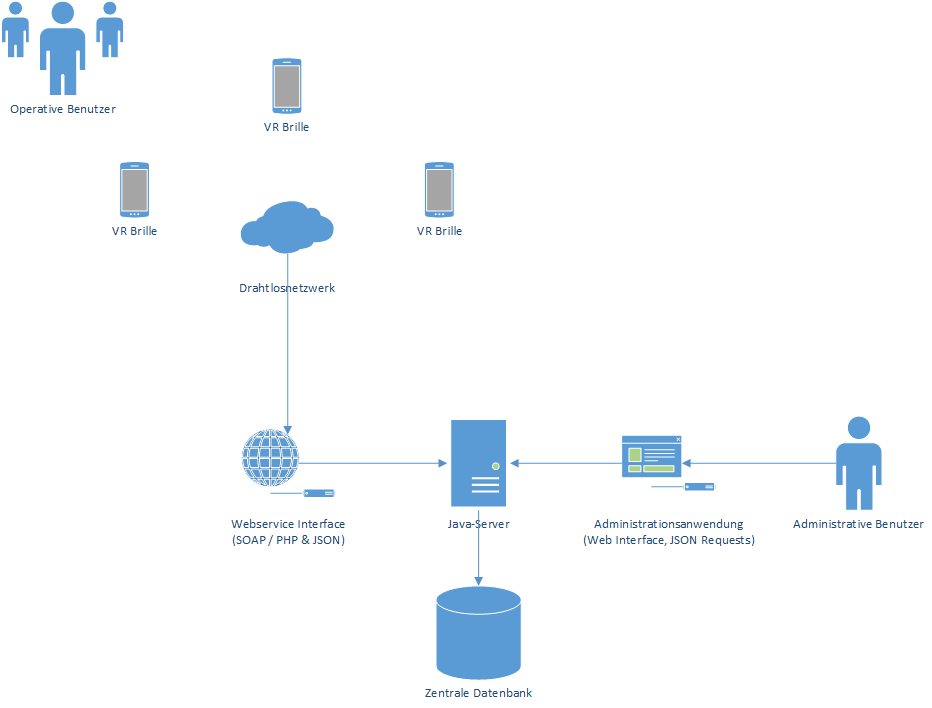
\includegraphics[width=\textwidth]{Bilder/Abbildungen/architektur_serverclient.png}}
	\caption{Schematische Darstellung der Server-Client-Architektur}
	\label{fig:architektur_serverclient}
\end{figure}

Im Folgenden werden die einzelnen Akteure mit ihren jeweiligen Komponenten genauer beschrieben.

\subsection{Server}

Der Server ist logisch in drei Komponenten unterteilt: einen Datenbankserver, und einen Webserver mit Web-Interface und \ac{REST} \ac{API}. Diese Komponenten müssen nicht zwingend auf dem selben Server bzw. auf dem selben Gerät installiert sein -- es kann es Sinn machen, ressourcenintensive Anwendungen auf weitere Geräte auszulagern. Gäbe es zum Beispiel sehr viele Clients, die viel Netzwerktraffic über die REST API erzeugen, wäre eine Auslagerung der API auf einen separaten Server bzw. Serverprozess denkbar, um die Performance der anderen Anwendungen nicht zu verringern. Ebenso wäre eine Auslagerung der Datenbank oder des Web-Interface möglich.

Der Einfachheit halber wird bei den folgenden Erläuterungen in dieser Arbeit davon ausgegangen, dass alle Komponenten auf dem selben Server liegen.

\subsubsection{Datenbankserver}
Der Datenbankserver (auch \ac{DBMS}) bildet die Kommunikationsschnittstelle, über die alle Anwendungen auf die Datenbank zugreifen. Die Datenbank selbst ist eine relationale \ac{SQL}-Datenbank, auf welche als \ac{DBMS} MySQL aufgesetzt wurde. Diese Entscheidung liegt darin begründet, dass für das Web-Interface und die REST API als serverseitige Scriptsprache \ac{PHP} gewählt wurde und dazu üblicherweise MySQL als DBMS verwendet wird, aufgrund der guten Kompatibilität und Bewährtheit.

\subsubsection{Web-Interface}
Das Web-Interface bildet die Administrationsoberfläche, über die das System gesteuert werden kann. Hier können die Benutzer des Systems sowie ihre Berechtigungen verwaltet werden. Außerdem bietet die Webadministration umfangreiche Möglichkeiten, um die Entitäten des Systems zu konfigurieren, wie z.B. Produkte oder Regale auf der Verkaufsfläche.

\subsubsection{Client-Schnittstelle}
Damit die Clients Daten aus der Datenbank abfragen oder ändern können, wird eine weitere Systemschnittstelle benötigt -- die Verwendung der Webadministration zur Datenmanipulation, z.B. über die Datenbrille, ist aus ergonomischen Gründen nicht geeignet, da die Brille über eingeschränkte Eingabemöglichkeiten verfügt und ohnehin über eine eigens entwickelte App mit Zusatzfunktionen wie z.B. Barcode-Scanner verfügt.

Die Schnittstelle stellt Dienste für alle Funktionen bereit, die von den Clients benötigt werden, z.B. einen Dienst zum Abruf von Produktinformationen, oder einen Dienst zum Aktualisieren des Warenbestandes. Das Kommunikationsverfahren und die bereitgestellten Dienste werden im Implementierungsteil dieser Arbeit erläutert.

\subsection{Clients}
Wie bereits in der Einführung der Architektur angedeutet, handelt es sich bei den Clients im System von SMAR um alle Geräte, die von operativen Benutzern im System verwendet werden: z.B. Smartphones, Tablets und -- im Fall dieser Arbeit mit besonderem Fokus -- Datenbrillen. Diese Geräte kommunizieren über das Netzwerk mit der REST API, um Lese- und Schreibzugriffe auf den Daten auszuführen.

\section{Datenbank-Architektur}
\label{sec:architektur_datenbank}

Der Entwurf der Datenbank erfordert besonders sorgsame Planung. Das Datenbankschema sollte künftige Erweiterungen der Software unterstützen und späteren Anpassungen am Schema möglichst vorbeugen, da sowohl das Web-Interface als auch die REST API auf dem Schema arbeiten und somit bei Änderung des Schemas auch weitreichende Änderungen im Quellcode die Folge wären (Anmerkung: für die App auf der Brille oder anderen Clients wären durch die Abstraktion über die REST API u.U. keine Anpassungen nötig).
Deshalb wurden bei der Planung der Datenbank für SMAR bereits Funktionen berücksichtigt, die in der dieser Arbeit zugrunde liegenden Version noch nicht implementiert sind, und entsprechende Tabellen und Spalten angelegt. Die grafische Übersicht veranschaulicht das Schema mit allen Tabellen, Spalten und Beziehungen von Feldern untereinander und wird im Folgenden näher erläutert:

\begin{figure}[H]
	\centering
	{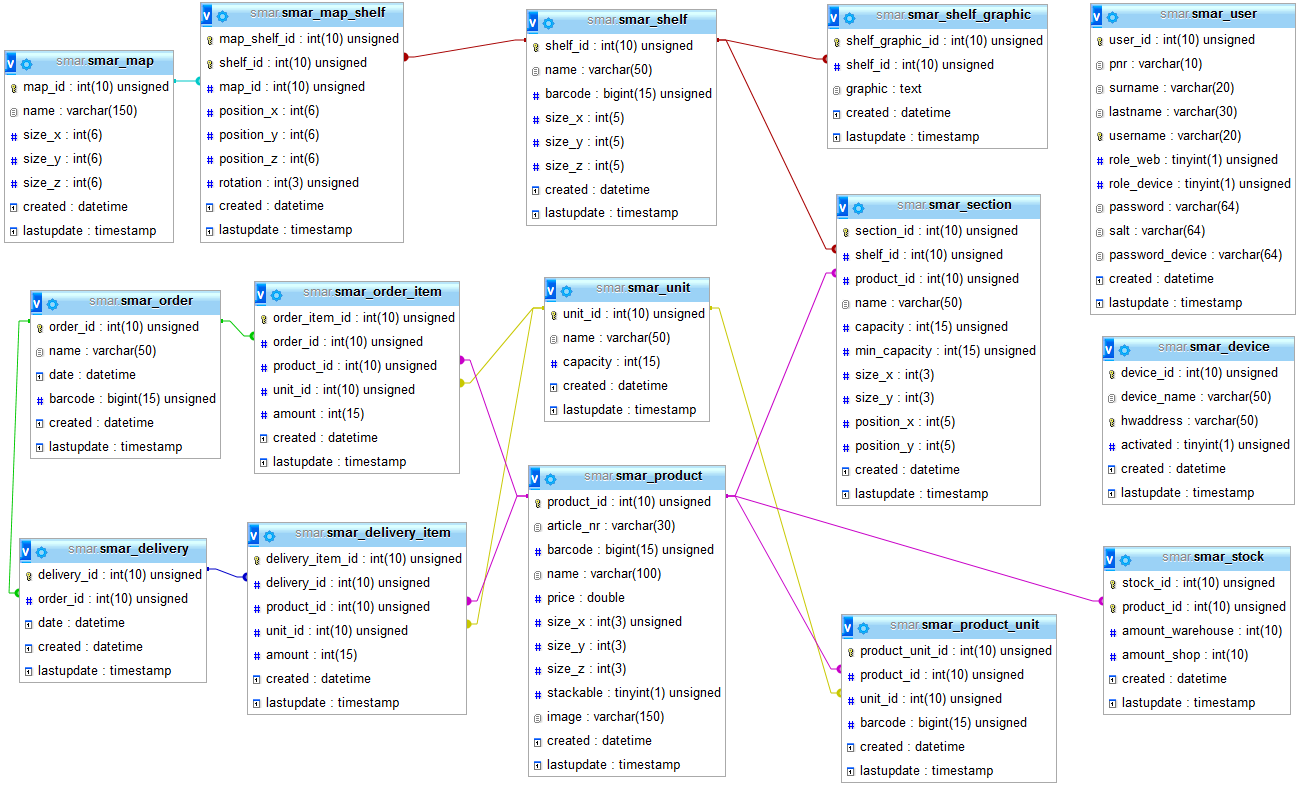
\includegraphics[width=\textwidth]{Bilder/Abbildungen/architektur_datenbankschema.png}}
	\caption{Tabellendefinitionen der Datenbank (Screenshot aus phpMyAdmin)}
	\label{fig:architektur_datenbankschema}
\end{figure}

Im Shelf Management drehen sich die grundlegenden Prozesse um Produkte -- dementsprechend gehört die Tabelle \textit{\textbf{product}} zu den umfangreichsten Tabellen. Hier werden alle wesentlichen Informationen zu einem Produkt gespeichert, z.B. Bezeichnung, Artikelnummer und Preis. Wichtig ist auch der abgespeicherte Barcode, über den das Produkt beim Scannen über die Brille identifiziert werden kann. Außerdem können die Maße des Produktes (Höhe, Breite, Tiefe) sowie die Stapelbarkeit (ja oder nein) angegeben werden -- diese Daten können bei der Lagerplatzberechnung interessant sein.\\

Mit der Tabelle \textit{\textbf{product}} sind weitere Tabellen logisch verknüpft. Sehr wichtig im Rahmen des Shelf Managements ist der Lagerbestand eines Produktes, welcher in der Tabelle \textit{\textbf{stock}} gespeichert wird. Konzeptionell ließe sich der Warenbestand direkt in \textit{\textbf{product}} speichern -- aus Gründen der Übersichtlichkeit und Performanz wurde die Speicherung vom Produkt logisch getrennt, da die Schreib- und Lesezugriffe auf den Warenbestand in der Anwendung oft isoliert erfolgen. Es können mehrere Bestände für ein Produkt erfasst werden: Bestand im Lager der Filiale (\textit{amount\_ warehouse}) und Bestand im Regal bzw. auf der Verkaufsfläche (\textit{amount\_ shop}). Diese Bestände werden entsprechend bei der Warenannahme, beim Einräumen in das Regal sowie an der Kasse beim Verkauf verändert. Prinzipiell können hier auch weitere Lagerorte hinzugefügt werden.\\

Produkte werden im Lager und im Shelf Management oft nicht nur einzeln, sondern auch in bestimmten größeren Mengen prozessiert, bspw. in Form von Kartons fester Größe; Produkte werden i.d.R. karton- oder sogar palettenweise bestellt und oft auch kartonweise auf der Verkaufsfläche eingeräumt. Für diesen Anwendungsfall können feste Produkteinheiten (\glqq units\grqq ) in der Tabelle \textit{\textbf{unit}} definiert werden. Die Beziehung zwischen einer Einheit und einem Produkt wird in \textit{\textbf{product\_ unit}} beschrieben. Diese Trennung der Produkt-Einheit-Beziehung ermöglicht eine Wiederverwendbarkeit von Produkteinheiten für mehrere Produkte. Jeder Produkt-Einheit-Beziehung kann ein eigener Barcode zugewiesen werden, sodass bspw. ein entsprechender Karton beim Scannen mit der Brille direkt erkannt werden kann.\\

Die Verwendung von Produkteinheiten ist grundsätzlich optional, da diese über Zusatzfunktionen der Software bzw. einen separaten Barcode angesprochen werden. Je nach Umsetzung im Handel haben z.B. Kartons entweder einen eigenen Barcode, oder den selben Barcode wie das Produkt, oder gar keinen Barcode; alle diese Fälle lassen sich mit diesem Datenbankschema abbilden und nutzen.\\

Neben dem Produkt ist das Verkaufsregal eine weitere wesentliche Entität im Shelf Management. Regale werden über die Tabelle \textit{\textbf{shelf}} definiert. Regale haben eine feste Größe (Höhe, Breite, Tiefe) und können ebenfalls über einen Barcode identifiziert werden.\\

Die Verbindung zwischen Regalen und Produkten bilden die Regalfächer (\glqq sections\grqq ) in der Tabelle \textit{\textbf{section}}. Ein Regalfach wird genau einem Regal zugeordnet und kann genau einen Produkttyp aufnehmen. Es werden die Größe des Fachs (Breite, Höhe) sowie die Position des Fachs im zugeordneten Regal (Abstand zu linker oberer Ecke als X/Y Koordinaten) abgespeichert. Außerdem ist die maximale Kapazität des Regals angegeben (also die höchstmögliche Befüllung mit dem zugeordneten Produkt), sowie optional ein Mindestfüllbestand. Letzterer kann verwendet werden, um im System anzuzeigen, welche Produkte aufgefüllt werden müssen, damit die entsprechenden Regalfächer nicht komplett leer werden.\\

Mit der Tabelle  \textit{\textbf{shelf}} sind ebenfalls noch weitere Tabellen verbunden. Die Tabelle  \textit{\textbf{shelf\_ graphic}} speichert vorgenerierte Grafiken der Regale im \ac{SVG}-Format, die von der App auf der Brille direkt verwendet werden können, um Rechenaufwand zu sparen. Um eine Wegfindung zu Regalen auf der Verkaufsfläche realisieren zu können, können in der Tabelle \textit{\textbf{map}} Verkaufsflächen definiert werden, sowie über die Tabelle \textit{\textbf{map\_ shelf}} Regale auf einer Verkaufsfläche angeordnet werden.\\

Um bei der Warenannahme die erhaltene Ware mit vorausgegangenen Bestellungen abgleichen zu können, müssen die Bestellungen im System hinterlegt sein. In der Tabelle \textit{\textbf{order}} können einzelne Bestellungen gespeichert werden, die zugehörigen Positionen liegen in der Tabelle \textit{\textbf{order\_ item}}, welche wiederum auf Entitäten der Tabellen  \textit{\textbf{product}} und \textit{\textbf{unit}} verweist.\\

Zuletzt sei auch die Tabelle \textit{\textbf{user}} genannt, welche wesentlich für die Sicherheit der Anwendung ist. Sie speichert alle Informationen zu den Benutzern des Systems: die Basisdaten zu einer Person, die Zugangsdaten für das Web-Interface und die Brille, sowie die jeweils zugeordneten Berechtigungen eines Benutzers.\\

